\documentclass[11pt,a4paper]{article}
\usepackage[utf8]{inputenc}\usepackage[T1]{fontenc}
\usepackage[margin=1in]{geometry}
\usepackage{amsmath,amssymb,booktabs,graphicx,enumitem,xcolor,parskip,titlesec}
\usepackage[hidelinks]{hyperref}
\graphicspath{{figures/}}
\definecolor{qnavy}{RGB}{20,40,75}\definecolor{qgrey}{RGB}{90,90,90}\definecolor{qred}{RGB}{150,30,30}
\titleformat{\section}{\large\bfseries\color{qnavy}}{\thesection}{0.6em}{}
\begin{document}\thispagestyle{empty}
\noindent
{\large\bfseries\color{qnavy} Report R10 --- What Is the KEAP1 Methylation Phenotype?}\\[2pt]
{\color{qgrey}Characterising R08's positive finding, and resolving the confound R08 declared
unresolvable.}\\[6pt]
{\color{qgrey}\rule{\textwidth}{0.4pt}}

\medskip
\noindent 7 August 2026 \quad\textbullet\quad Quantara

\section*{Summary}

R08 reported that 29.4\% of probes are differentially methylated by KEAP1 mutation status within
lung adenocarcinoma. That is a statistical statement with no biological content, and R08 left
its main caveat open: it could not rule out that the phenotype was really a smoking signature.
This report addresses both, using all 392{,}489 retained probes rather than R08's 20{,}000
sample.

\textbf{The phenotype is strong.} A nested cross-validated classifier predicts KEAP1 mutation
status from methylation alone at \textbf{AUROC 0.910} (95\% CI 0.869--0.946) in 471 tumours with
84 mutants. The sex positive control through the identical pipeline reaches 1.000, and the result
is stable across five seeds (0.868--0.910).

\textbf{It is not a smoking signature.} This was R08's declared-unresolvable limitation, and it
turned out to be resolvable from the other direction. Defining the smoking signature in
KEAP1-\emph{wildtype} tumours only --- which needs no never-smokers carrying the mutation ---
gives 37{,}008 probes, of which only \textbf{14{,}306 are shared} with the 115{,}557-probe KEAP1
signature. That is 12.4\% of the KEAP1 signature and just \textbf{1.31$\times$} what two
independent signatures of these sizes would share by chance. Deleting every smoking-shared probe
and retraining leaves the classifier at \textbf{AUROC 0.904}.

\textbf{It has a coherent genomic structure.} Differential probes are \emph{depleted} in promoter
CpG islands (21.5\%, OR 0.54) and at transcription start sites (TSS200: 18.7\%, OR 0.51), and
\emph{enriched} in open sea (34.6\%, OR 1.44), island shelves (OR 1.26--1.27) and intergenic
regions (OR 1.66). This is distal and gene-body remodelling, not promoter silencing.

\textbf{The pre-declared NRF2 pathway is enriched} --- and this was a genuine test, not a
foregone conclusion. KEAP1 loss activates NRF2 post-translationally, which does not by itself
predict any methylation change at NRF2 targets, so the prior was declared weak in advance. The
33 NRF2-pathway genes on the array average 35.7\% of probes differential against a
probe-count-matched null of 23.9\% ($p = 0.003$).

\section{Q1 --- how strong is it?}

\begin{center}
\begin{tabular}{@{}lrr@{}}
\toprule
& \textbf{AUROC} & \textbf{95\% CI} \\
\midrule
Sex (positive control, same pipeline) & 1.000 & 1.000--1.000 \\
\textbf{KEAP1 mutation status} & \textbf{0.910} & 0.869--0.946 \\
KEAP1, after deleting all 37{,}008 smoking-shared probes & 0.904 & --- \\
\midrule
Across 5 cross-validation seeds & \multicolumn{2}{r}{median 0.898, range 0.868--0.910} \\
\bottomrule
\end{tabular}
\end{center}

\noindent 471 LUAD primary tumours, 84 KEAP1-mutant. LUSC was excluded entirely, because R08
established that pooling histologies confounds every comparison of this kind. Probe selection
and hyperparameters were fitted strictly inside training folds.

The signature itself reproduces R08 almost exactly: 29.44\% of all 392{,}489 probes against
R08's 29.35\% from a 20{,}000-probe sample, so R08's sampling error was negligible.

\begin{center}
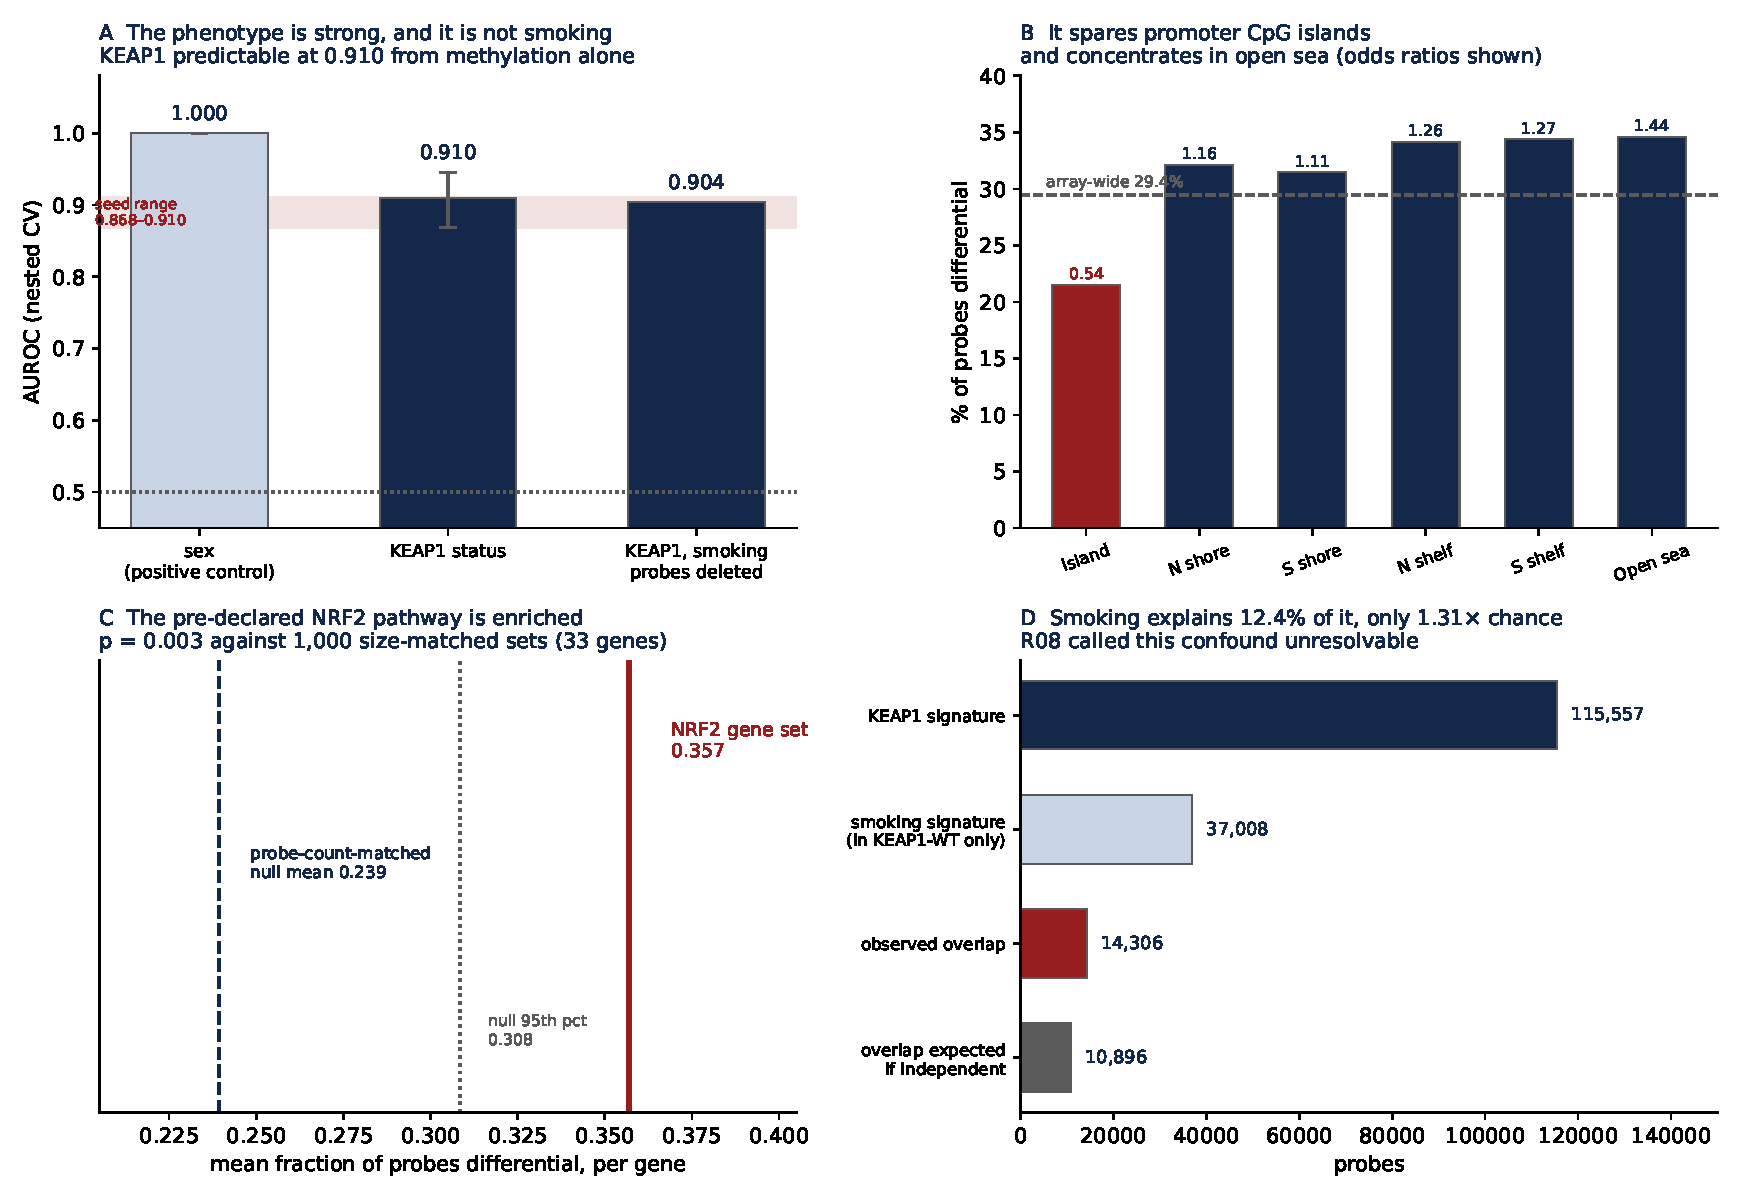
\includegraphics[width=\textwidth]{r10_panels.pdf}
\end{center}
\noindent{\small\color{qgrey}\textbf{A} Classifier performance, with the sex control and the
smoking-deleted variant; shaded band is the 5-seed range. \textbf{B} Differential probes by CpG
island context, odds ratios above each bar; red marks depletion. \textbf{C} The NRF2 gene set
against 1{,}000 probe-count-matched random sets. \textbf{D} The overlap with smoking, against
what chance alone would give.}

\section{Q2 --- where in the genome?}

\begin{center}
\begin{tabular}{@{}lrrr@{}}
\toprule
\textbf{Context} & \textbf{Probes} & \textbf{\% differential} & \textbf{Odds ratio} \\
\midrule
CpG island        & 134{,}053 & 21.5\% & \textbf{0.54} \\
North shore       & \phantom{0}52{,}248 & 32.1\% & 1.16 \\
South shore       & \phantom{0}40{,}841 & 31.5\% & 1.11 \\
North shelf       & \phantom{0}18{,}409 & 34.2\% & 1.26 \\
South shelf       & \phantom{0}16{,}371 & 34.4\% & 1.27 \\
Open sea          & 130{,}567 & 34.6\% & \textbf{1.44} \\
\midrule
\multicolumn{4}{@{}l}{\textit{by gene region}} \\
TSS200            & --- & 18.7\% & \textbf{0.51} \\
TSS1500           & --- & 27.2\% & 0.88 \\
Gene body         & --- & 31.0\% & 1.12 \\
Intergenic (unannotated) & --- & 38.0\% & \textbf{1.66} \\
\bottomrule
\end{tabular}
\end{center}

\noindent Array-wide baseline is 29.4\%; 390{,}543 of the 392{,}489 probes (99.5\%) carry
manifest annotation, so coverage is not a limitation here. The gradient is monotonic and unambiguous: the further
from a promoter CpG island, the more likely a probe is differential. Whatever KEAP1 mutation
associates with epigenetically, it is not classical promoter hypermethylation.

\section{Q3 --- which genes?}

Of the 39 pre-declared NRF2/KEAP1-pathway genes, 33 have at least five probes on the array.

\begin{center}
\begin{tabular}{@{}lr@{}}
\toprule
NRF2 pathway, mean fraction of probes differential & 0.357 \\
Unmatched random null (1{,}000 sets), mean & 0.243 \quad ($p = 0.006$) \\
Probe-count-matched null (1{,}000 sets), mean & 0.239 \quad ($\mathbf{p = 0.003}$) \\
Null 95th percentile & 0.308 \\
\bottomrule
\end{tabular}
\end{center}

The audit re-ran the null matched on probes-per-gene, because random sets matched only on gene
count would confound gene size with the result. The enrichment strengthened rather than weakened
($p$ 0.006 $\rightarrow$ 0.003), and probes-per-gene correlates only weakly with the
differential fraction in any case (Spearman $\rho = 0.089$).

Among genes with $\geq$10 probes, the most completely differential include \textit{GATA5},
\textit{LZTS1}, \textit{UNCX}, \textit{NCAN} and \textit{GPX6} --- developmental transcription
factors and known methylation-regulated loci. This list is descriptive only: the ranking favours
genes with dense probe coverage, and no gene-level claim is made from it.

\section{Q4 --- is it really smoking?}

R08 stated this confound could not be resolved, because only 4 of 81 never-smokers carried a
KEAP1 mutation, so no never-smoker stratum could support a genome-wide test. That framing assumed
the test had to hold smoking constant. Reversing it removes the constraint: define the smoking
signature among KEAP1-\emph{wildtype} tumours (308 ever-smokers vs 65 never-smokers), then ask
how much of the KEAP1 signature consists of those same probes.

\begin{center}
\begin{tabular}{@{}lr@{}}
\toprule
KEAP1 signature & 115{,}557 probes \\
Smoking signature (in KEAP1-wildtype tumours only) & \phantom{0}37{,}008 probes \\
Observed overlap & \phantom{0}14{,}306 \\
Overlap expected if the two were independent & \phantom{0}10{,}896 \\
\midrule
Observed / expected & \textbf{1.31$\times$} \\
Share of the KEAP1 signature that is smoking-shared & \textbf{12.4\%} \\
Jaccard index & 0.104 \\
Classifier AUROC after deleting all shared probes & \textbf{0.904} (from 0.910) \\
\quad{\small(355{,}481 of 392{,}489 probes retained)} & \\
\bottomrule
\end{tabular}
\end{center}

The two signatures are barely more similar than chance, and the classifier is indifferent to
losing every probe they share. \textbf{The KEAP1 methylation phenotype is its own.}

\textbf{The residual caveat, stated rather than hidden.} The smoking comparison rests on 65
never-smokers, so the smoking signature is measured with less precision than its 37{,}008 probes
suggests. If it is systematically under-detected, the true overlap is larger than 12.4\%. Two
things bound that concern: the limiting group sizes are comparable (65 never-smokers against 84
KEAP1 mutants), so the two signatures are not grossly unequally powered; and the deletion
experiment in the audit does not depend on the smoking signature being complete --- removing
37{,}008 candidate probes cost 0.006 AUROC.

\section{What this changes}

\begin{itemize}[leftmargin=1.2em,itemsep=2pt]
\item \textbf{R08's positive finding is upgraded from statistical to characterised.} ``29\% of
probes differ'' becomes: AUROC 0.910, distal and intergenic rather than promoter-based,
NRF2-enriched, and independent of smoking.
\item \textbf{R08's limitation 3 is resolved, not merely acknowledged.} It was resolvable by
inverting the design. That is worth noting for the other open confounds in this series.
\item \textbf{The prognostic conclusion is unchanged.} R08 showed methylation adds nothing to
mutation, stage and age for survival (LR $p = 0.85$), and nothing here revisits that. A strong
biological phenotype and no prognostic value are not in conflict --- KEAP1 mutation status is
already known, so predicting it from a more expensive assay has no clinical use on its own.
\item \textbf{Where it could matter.} The distal, NRF2-enriched pattern is a mechanistic lead
about how KEAP1 loss reshapes the epigenome, and it is measurable in archival tissue. Whether it
tracks NRF2 pathway \emph{activity} --- as opposed to KEAP1 genotype --- is the natural next
question, and needs matched expression data rather than more methylation.
\end{itemize}

\section{Reproducing this report}

\begin{itemize}[leftmargin=1.2em,itemsep=1pt]
\item Analysis: \texttt{evidence/m11\_keap1\_phenotype.py}; audit:
      \texttt{evidence/audit\_m11.py}
\item Config hash, written before any outcome was read:
      \texttt{229f8cb6cc4312e8\ldots1960db0f80}. The NRF2 gene set is listed inside it, fixed
      before any enrichment was computed
\item Annotation: Illumina HumanMethylation450 v1.1 manifest, GEO GPL13534 supplementary file
\item \texttt{evidence/keap1\_signature\_qvalues.csv.gz} --- every one of the 115{,}557
      significant probes with its $q$-value, so the signature can be re-used or checked directly
\item Beta matrix: \texttt{gs://heydonto-quantara-lungcdx/data-request-2026-08/lung/}
      \texttt{tcga\_methylation\_450k/} (see R08)
\item Figure: \texttt{python3 make\_figure.py}
\end{itemize}

\end{document}
